\documentclass[conference]{IEEEtran}
% Some Computer Society conferences also require the compsoc mode option,
% but others use the standard conference format.
%
% If IEEEtran.cls has not been installed into the LaTeX system files,
% manually specify the path to it like:
% \documentclass[conference]{../sty/IEEEtran}

\usepackage[utf8]{inputenc}

% *** MISC UTILITY PACKAGES ***
%
\usepackage{ifpdf}
% Heiko Oberdiek's ifpdf.sty is very useful if you need conditional
% compilation based on whether the output is pdf or dvi.
% usage:
 \ifpdf
   % pdf code
 \else
   % dvi code
 \fi




\usepackage[ngerman]{babel}
%\usepackage{ngerman}

%\usepackage{breakurl}




% *** CITATION PACKAGES ***
%
\usepackage{cite}
% cite.sty was written by Donald Arseneau
% V1.6 and later of IEEEtran pre-defines the format of the cite.sty package
% \cite{} output to follow that of the IEEE. Loading the cite package will
% result in citation numbers being automatically sorted and properly
% "compressed/ranged". e.g., [1], [9], [2], [7], [5], [6] without using
% cite.sty will become [1], [2], [5]--[7], [9] using cite.sty. cite.sty's
% \cite will automatically add leading space, if needed. Use cite.sty's
% noadjust option (cite.sty V3.8 and later) if you want to turn this off
% such as if a citation ever needs to be enclosed in parenthesis.
% cite.sty is already installed on most LaTeX systems. Be sure and use
% version 5.0 (2009-03-20) and later if using hyperref.sty.
% The latest version can be obtained at:
% http://www.ctan.org/pkg/cite
% The documentation is contained in the cite.sty file itself.






% *** GRAPHICS RELATED PACKAGES ***
%
\ifCLASSINFOpdf
  \usepackage[pdftex]{graphicx}
  % declare the path(s) where your graphic files are
  % \graphicspath{{../pdf/}{../jpeg/}}
  % and their extensions so you won't have to specify these with
  % every instance of \includegraphics
  % \DeclareGraphicsExtensions{.pdf,.jpeg,.png}
\else
  % or other class option (dvipsone, dvipdf, if not using dvips). graphicx
  % will default to the driver specified in the system graphics.cfg if no
  % driver is specified.
  % \usepackage[dvips]{graphicx}
  % declare the path(s) where your graphic files are
  % \graphicspath{{../eps/}}
  % and their extensions so you won't have to specify these with
  % every instance of \includegraphics
  % \DeclareGraphicsExtensions{.eps}
\fi
% graphicx was written by David Carlisle and Sebastian Rahtz. It is
% required if you want graphics, photos, etc. graphicx.sty is already
% installed on most LaTeX systems. The latest version and documentation
% can be obtained at: 
% http://www.ctan.org/pkg/graphicx
% Another good source of documentation is "Using Imported Graphics in
% LaTeX2e" by Keith Reckdahl which can be found at:
% http://www.ctan.org/pkg/epslatex
%
% latex, and pdflatex in dvi mode, support graphics in encapsulated
% postscript (.eps) format. pdflatex in pdf mode supports graphics
% in .pdf, .jpeg, .png and .mps (metapost) formats. Users should ensure
% that all non-photo figures use a vector format (.eps, .pdf, .mps) and
% not a bitmapped formats (.jpeg, .png). The IEEE frowns on bitmapped formats
% which can result in "jaggedy"/blurry rendering of lines and letters as
% well as large increases in file sizes.
%
% You can find documentation about the pdfTeX application at:
% http://www.tug.org/applications/pdftex





% *** MATH PACKAGES ***
%
%\usepackage{amsmath}
% A popular package from the American Mathematical Society that provides
% many useful and powerful commands for dealing with mathematics.
%
% Note that the amsmath package sets \interdisplaylinepenalty to 10000
% thus preventing page breaks from occurring within multiline equations. Use:
%\interdisplaylinepenalty=2500
% after loading amsmath to restore such page breaks as IEEEtran.cls normally
% does. amsmath.sty is already installed on most LaTeX systems. The latest
% version and documentation can be obtained at:
% http://www.ctan.org/pkg/amsmath





% *** SPECIALIZED LIST PACKAGES ***
%
%\usepackage{algorithmic}
% algorithmic.sty was written by Peter Williams and Rogerio Brito.
% This package provides an algorithmic environment fo describing algorithms.
% You can use the algorithmic environment in-text or within a figure
% environment to provide for a floating algorithm. Do NOT use the algorithm
% floating environment provided by algorithm.sty (by the same authors) or
% algorithm2e.sty (by Christophe Fiorio) as the IEEE does not use dedicated
% algorithm float types and packages that provide these will not provide
% correct IEEE style captions. The latest version and documentation of
% algorithmic.sty can be obtained at:
% http://www.ctan.org/pkg/algorithms
% Also of interest may be the (relatively newer and more customizable)
% algorithmicx.sty package by Szasz Janos:
% http://www.ctan.org/pkg/algorithmicx




% *** ALIGNMENT PACKAGES ***
%
%\usepackage{array}
% Frank Mittelbach's and David Carlisle's array.sty patches and improves
% the standard LaTeX2e array and tabular environments to provide better
% appearance and additional user controls. As the default LaTeX2e table
% generation code is lacking to the point of almost being broken with
% respect to the quality of the end results, all users are strongly
% advised to use an enhanced (at the very least that provided by array.sty)
% set of table tools. array.sty is already installed on most systems. The
% latest version and documentation can be obtained at:
% http://www.ctan.org/pkg/array


% IEEEtran contains the IEEEeqnarray family of commands that can be used to
% generate multiline equations as well as matrices, tables, etc., of high
% quality.




% *** SUBFIGURE PACKAGES ***
%\ifCLASSOPTIONcompsoc
%  \usepackage[caption=false,font=normalsize,labelfont=sf,textfont=sf]{subfig}
%\else
%  \usepackage[caption=false,font=footnotesize]{subfig}
%\fi
% subfig.sty, written by Steven Douglas Cochran, is the modern replacement
% for subfigure.sty, the latter of which is no longer maintained and is
% incompatible with some LaTeX packages including fixltx2e. However,
% subfig.sty requires and automatically loads Axel Sommerfeldt's caption.sty
% which will override IEEEtran.cls' handling of captions and this will result
% in non-IEEE style figure/table captions. To prevent this problem, be sure
% and invoke subfig.sty's "caption=false" package option (available since
% subfig.sty version 1.3, 2005/06/28) as this is will preserve IEEEtran.cls
% handling of captions.
% Note that the Computer Society format requires a larger sans serif font
% than the serif footnote size font used in traditional IEEE formatting
% and thus the need to invoke different subfig.sty package options depending
% on whether compsoc mode has been enabled.
%
% The latest version and documentation of subfig.sty can be obtained at:
% http://www.ctan.org/pkg/subfig




% *** FLOAT PACKAGES ***
%
%\usepackage{fixltx2e}
% fixltx2e, the successor to the earlier fix2col.sty, was written by
% Frank Mittelbach and David Carlisle. This package corrects a few problems
% in the LaTeX2e kernel, the most notable of which is that in current
% LaTeX2e releases, the ordering of single and double column floats is not
% guaranteed to be preserved. Thus, an unpatched LaTeX2e can allow a
% single column figure to be placed prior to an earlier double column
% figure.
% Be aware that LaTeX2e kernels dated 2015 and later have fixltx2e.sty's
% corrections already built into the system in which case a warning will
% be issued if an attempt is made to load fixltx2e.sty as it is no longer
% needed.
% The latest version and documentation can be found at:
% http://www.ctan.org/pkg/fixltx2e


%\usepackage{stfloats}
% stfloats.sty was written by Sigitas Tolusis. This package gives LaTeX2e
% the ability to do double column floats at the bottom of the page as well
% as the top. (e.g., "\begin{figure*}[!b]" is not normally possible in
% LaTeX2e). It also provides a command:
%\fnbelowfloat
% to enable the placement of footnotes below bottom floats (the standard
% LaTeX2e kernel puts them above bottom floats). This is an invasive package
% which rewrites many portions of the LaTeX2e float routines. It may not work
% with other packages that modify the LaTeX2e float routines. The latest
% version and documentation can be obtained at:
% http://www.ctan.org/pkg/stfloats
% Do not use the stfloats baselinefloat ability as the IEEE does not allow
% \baselineskip to stretch. Authors submitting work to the IEEE should note
% that the IEEE rarely uses double column equations and that authors should try
% to avoid such use. Do not be tempted to use the cuted.sty or midfloat.sty
% packages (also by Sigitas Tolusis) as the IEEE does not format its papers in
% such ways.
% Do not attempt to use stfloats with fixltx2e as they are incompatible.
% Instead, use Morten Hogholm'a dblfloatfix which combines the features
% of both fixltx2e and stfloats:
%
% \usepackage{dblfloatfix}
% The latest version can be found at:
% http://www.ctan.org/pkg/dblfloatfix




% *** PDF, URL AND HYPERLINK PACKAGES ***
%
%\usepackage{url}
% url.sty was written by Donald Arseneau. It provides better support for
% handling and breaking URLs. url.sty is already installed on most LaTeX
% systems. The latest version and documentation can be obtained at:
% http://www.ctan.org/pkg/url
% Basically, \url{my_url_here}.
\usepackage[hyphens]{url}



% *** Do not adjust lengths that control margins, column widths, etc. ***
% *** Do not use packages that alter fonts (such as pslatex).         ***
% There should be no need to do such things with IEEEtran.cls V1.6 and later.
% (Unless specifically asked to do so by the journal or conference you plan
% to submit to, of course. )


% correct bad hyphenation here
\hyphenation{op-tical net-works semi-conduc-tor}


\begin{document}
%

\title{Cloud Computing DNS Dienst: Route 53}


\author{\IEEEauthorblockN{Andreas Leopold N\"uchter}
\IEEEauthorblockA{Hochschule f\"ur angewandte Wissenschaften W\"urzburg-Schweinfurt\\
Fakult\"at Informatik und Wirtschaftsinformatik.\\
Hausarbeit zum Abschluss des Seminars Cloud Computing\\
Email: an.nuechter@gmail.com}}




% make the title area
\maketitle


\begin{abstract}
Der Abstract kommt irgendwann Später
\end{abstract}

% no keywords



\section{Einführung}
\IEEEPARstart{T}{his} demo file is intended to serve as a ``starter file''
for IEEE conference papers produced under \LaTeX\ using
IEEEtran.cls version 1.8b and later.
I wish you the best of success.

\hfill mds
 
\hfill August 26, 2015


% An example of a floating figure using the graphicx package.
% Note that \label must occur AFTER (or within) \caption.
% For figures, \caption should occur after the \includegraphics.
% Note that IEEEtran v1.7 and later has special internal code that
% is designed to preserve the operation of \label within \caption
% even when the captionsoff option is in effect. However, because
% of issues like this, it may be the safest practice to put all your
% \label just after \caption rather than within \caption{}.
%
% Reminder: the "draftcls" or "draftclsnofoot", not "draft", class
% option should be used if it is desired that the figures are to be
% displayed while in draft mode.
%
%\begin{figure}[!t]
%\centering
%\includegraphics[width=2.5in]{myfigure}
% where an .eps filename suffix will be assumed under latex, 
% and a .pdf suffix will be assumed for pdflatex; or what has been declared
% via \DeclareGraphicsExtensions.
%\caption{Simulation results for the network.}
%\label{fig_sim}
%\end{figure}

% Note that the IEEE typically puts floats only at the top, even when this
% results in a large percentage of a column being occupied by floats.


% An example of a double column floating figure using two subfigures.
% (The subfig.sty package must be loaded for this to work.)
% The subfigure \label commands are set within each subfloat command,
% and the \label for the overall figure must come after \caption.
% \hfil is used as a separator to get equal spacing.
% Watch out that the combined width of all the subfigures on a 
% line do not exceed the text width or a line break will occur.
%
%\begin{figure*}[!t]
%\centering
%\subfloat[Case I]{\includegraphics[width=2.5in]{box}%
%\label{fig_first_case}}
%\hfil
%\subfloat[Case II]{\includegraphics[width=2.5in]{box}%
%\label{fig_second_case}}
%\caption{Simulation results for the network.}
%\label{fig_sim}
%\end{figure*}
%
% Note that often IEEE papers with subfigures do not employ subfigure
% captions (using the optional argument to \subfloat[]), but instead will
% reference/describe all of them (a), (b), etc., within the main caption.
% Be aware that for subfig.sty to generate the (a), (b), etc., subfigure
% labels, the optional argument to \subfloat must be present. If a
% subcaption is not desired, just leave its contents blank,
% e.g., \subfloat[].


% An example of a floating table. Note that, for IEEE style tables, the
% \caption command should come BEFORE the table and, given that table
% captions serve much like titles, are usually capitalized except for words
% such as a, an, and, as, at, but, by, for, in, nor, of, on, or, the, to
% and up, which are usually not capitalized unless they are the first or
% last word of the caption. Table text will default to \footnotesize as
% the IEEE normally uses this smaller font for tables.
% The \label must come after \caption as always.
%
%\begin{table}[!t]
%% increase table row spacing, adjust to taste
%\renewcommand{\arraystretch}{1.3}
% if using array.sty, it might be a good idea to tweak the value of
% \extrarowheight as needed to properly center the text within the cells
%\caption{An Example of a Table}
%\label{table_example}
%\centering
%% Some packages, such as MDW tools, offer better commands for making tables
%% than the plain LaTeX2e tabular which is used here.
%\begin{tabular}{|c||c|}
%\hline
%One & Two\\
%\hline
%Three & Four\\
%\hline
%\end{tabular}
%\end{table}


% Note that the IEEE does not put floats in the very first column
% - or typically anywhere on the first page for that matter. Also,
% in-text middle ("here") positioning is typically not used, but it
% is allowed and encouraged for Computer Society conferences (but
% not Computer Society journals). Most IEEE journals/conferences use
% top floats exclusively. 
% Note that, LaTeX2e, unlike IEEE journals/conferences, places
% footnotes above bottom floats. This can be corrected via the
% \fnbelowfloat command of the stfloats package.



\section{Domain Name System}

Das Internet ist ohne die Technologie des \emph{Domain Name Systems}, im folgenden mit DNS abgekürzt, kaum noch vorstellbar. Über diesen Service ist es möglich für den Menschen einfach lesbare, alphabetische Namen, statt mehrstellige Nummern zu nutzen, um Ressourcen in einem Netzwerk aufzurufen und auf diese zuzugreifen. Diese alphanumerischen Namen werden ebenfalls als \emph{Domain Names} bezeichnet. Das Routing in einem großen Netzwerk wie dem Internet wäre jedoch schwer über solche Namen zu realisieren, stattdessen werden hierzu numerische IP-Adressen verwendet. Um trotzdem die besser nutzbaren alphabetischen Ausdrücke nutzen zu können ist also ein Service zur Übersetzung dieser in IP-Adressen gefordert. Früher mussten die IP und der zugehörige Domain Name lokal und manuell in einer Datei namens \textit{hosts} gespeichert werden. Mit dem enormen Wachstums des Internets musste jedoch eine neue Möglichkeit geschaffen werden. Diese Technologie bezeichnet man als \emph{Domain Name System}. \cite{Schreiner.2016}

Das im vorherigen Absatz beschriebene bedeutet, jedes Mal wenn der Domain Name einer Netzwerkressource, wie eines Webservers, eingegeben wird, muss diese zunächst in das IP-System übersetzt werden. Die Auflösung des Domain Namens kann jedoch nicht durch die reine Übersetzung der Zeichen erfolgen. Die Funktionsweise der Auflösung gleicht mehr der Verwendung eines Telefonbuchs. Auf einem DNS-Server ist eine Tabelle hinterlegt. Jede Zeile in dieser Tabelle besteht aus mindestens zwei Werten und wird als Record bezeichnet. Dem Domain Namen und der dazugehörigen IP-Adresse. Wird über einen sogenannten DNS-Lookup ein Domain Name angefragt, kann nun als Antwort die passende IP-Adresse zurückgegeben werden, über welche die erfragte Ressource erreicht werden kann.

\subsection{Domain-Namespace}
Der sogenannte Domain-Namespace (englisch für Namensraum) ist in einer Baumstruktur gegliedert und in unterschiedliche Zonen aufgeteilt. Der Wurzelknoten des Baumes stellt der Root-Knoten dar. Dieser wird durch einen Punkt symbolisiert. An erster Stelle nach dem Root-Knoten stehen die sogenannten Top-Level-Domains (TLD). Die am meisten verwendeten TLDs, laut einer Statistik vom Mai 2018, sind \textit{com} für \textit{Commercial} mit 46,5\% und darauf folgend, der für \textit{Organisation} stehende Eintrag, \textit{org} mit 5,1\% \cite{w3techs.2018}. Diese Top-Level-Domains werden auch als \textit{generic Top-Level-Domains(gTDL}) bezeichnet, da sie einen länderübergreifenden Code darstellen. Zusätzlich gibt es noch Top-Level-Domains, die einen Ländercode repräsentieren. Die meist verwendete länderspezifische TLD oder auch ccTLD (country code top-level-domain) ist hierbei die russische \textit{ru} und auch die für Deutschland stehende \textit{de} findet häufige Verwendung. \cite{IndianaUniversity.14.05.2018} 

Die Second-Level-Domain (SLD) befindet sich hierarchisch unter der Ebene der TLD. Sie wird häufig als frei wählbarer Name der Domain bezeichnet. Die einzelnen Hierarchiestufen werden von unten nach oben geschrieben und durch einen Punkt getrennt. Diese Schreibweise wird auch als \textit{Fully-Qualified Host Name} auf deutsch \textit{vollständig angegebener Rechnername}, bezeichnet. Ein Beispiel wäre hierfür die offizielle Adresse der Homepage der Hochschule \textit{fhws.de}, wobei fhws die SLD darstellt. Der Punkt, welcher den Root-Knoten repräsentiert wird meist weggelassen. Die auf die Second-Level-Domain folgenden Ebenen in der Baumstruktur werden auch als Sub-Domains bezeichnet. Diese dienen dem SLD Besitzer meist dazu unterschiedliche Services anzubieten oder eben direkt auf eine Netzwerkressource zuzugreifen. \cite{Schreiner.2016} \cite{1und1.2018} 

Ein vereinfachtes Beispiel einer solchen Struktur ist in Abbildung \ref{fig:DNSTree} unter Verwendung der Domain \textit{mail.google.com} zu sehen. Diese Domain führt auf den E-Mail Service von Google. Als weiteres Beispiel stellt der Domain-Name \textit{de.wikipedia.org} dar. Nachdem unter \textit{en.wikipedia.org} die englische Version der Wikipedia Website zu finden ist, bietet die Third-Level-Domain \textit{de} in dem Beispiel die Möglichkeit auf die deutsche Variante der Wissensdatenbank Wikipedia zu gelangen.

\begin{figure}[ht]
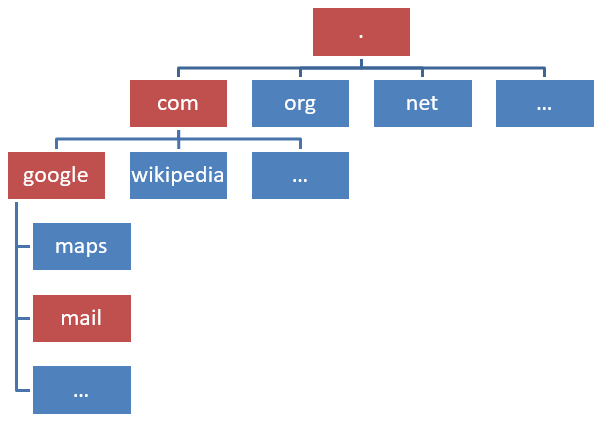
\includegraphics[width=\columnwidth]{images/dnsTree.png}
\caption{Beispiel der Domain mail.google.com in Baumstruktur}
\label{fig:DNSTree}
\end{figure}

\subsection{DNS-Server}
Die Anzahl an Domain-Names ist enorm groß und die Namensauflösung wäre wirtschaftlich kaum über allwissende DNS-Server realisierbar. Deshalb ist der Namensraum in unterschiedliche, von einander unabhängige Zonen aufgeteilt und als verteiltes System über mehrere sogenannte Nameserver realisiert. Diese dezentrale Verwaltung des Namensraums ermöglicht eine Lastverteilung und gewährleistet ebenfalls  eine bessere Ausfallsicherheit durch multiple Redundanzen im gesamten Netzwerk. 

Bei DNS-Servern unterscheidet man zwischen zwei Typen. Jede Zone enthält mindestens einen \textit{Autoritativen DNS-Server}. Dieser repräsentiert seine Zone und verwaltet lediglich orginale und definitive Einträge. Der Autoritative DNS-Server speichert keine Routing Informationen über andere Zonen und liefert nur eine Antwort auf Records die er tatsächlich selbst besitzt. Autoritative DNS-Server sind meist in einem Servercluster organisiert und der Master wird mehrfach durch andere Slave-Nameserver gespiegelt um Lastverteilung und Ausfallsicherheit zu gewährleisten. 

Im Gegensatz dazu steht der Nicht-autoritative DNS-Server. Dieser wiederum speichert zuvor durchgeführte DNS-Namensauflösungen. Er enthält somit nicht nur Informationen zu der Zone in der er sich befindet, sondern ebenfalls Datensätze aus zweiter oder dritter Hand. Erhält er eine Anfrage bezüglich einer Domain, zu der er keine Antwort liefern kann, übernimmt der Nameserver die Arbeit der weiteren Namensauflösung. Ist er bei der geforderten zuweisung des Domain-Namens erfolgreich, gibt er das Ergebnis zurück an den Auftraggeber und speichert dieses in seinem Arbeitsspeicher für zukünftige Anfragen. Da sich die Einträge in den fremden Namensräumen jedoch jederzeit verändern können, erhält jeder Eintrag seine eigene Time-to-live. Läuft diese ab muss der fremde Datensatz aus dem Speicher entfernt werden. Informationen, die ein Nicht-autoritativer DNS-Server hält, werden ebenfalls als \textit{nicht gesichert} angesehen. \cite{1und1.2018}

\subsection{DNS-Lookup}
Der Aufbau des DNS in einem dezentralen Datenbanksystem erschwert die Auflösung im Gegensatz zu einer zentralen Lösung, da die Informationen nicht an einem Ort durch eine einzelne Abfrage gefunden werden können. Wird nun, zum Beispiel durch die Eingabe einer URL in den Browser, ein DNS-Lookup angestoßen, so übernimmt zunächst der Betriebssystem interne Resolver die Aufgabe. Dieser Resolver speichert die zugehörigen IP Adressen zu den angefragten Domain-Names im Cache und liefert der Client-Anwendung den zugehörigen Wert direkt zurück. Ist der Eintrag nicht im Zwischenspeicher vorzufinden, so wird eine neue Anfrage an den nächsten DNS-Server vom Resolver generiert. Befindet sich im eigenen Netzwerk ein Nameserver, so wird dieser die Anfrage versuchen aufzulösen, ansonsten ist als nächste Instanz meist der DNS-Server des Internetdienstleisters eingetragen. Dieser gleicht die Anfrage mit seinen Datenbeständen ab und liefert die angefragte IP-Adresse bei Erfolg zurück an den Resolver. \cite{1und1.22.01.2018}

Kann der gesuchte Datensatz hier nicht gefunden werden kontaktiert der DNS-Server einen Root-Server. Dieser verwaltet, wie zuvor beschrieben, die Adressen für die TLDs. Der Root-Server kümmert sicher nicht selbst um die weitere Namensauflösung, sondern liefert dem anfragenden Nameserver lediglich einen Hinweis wo der angefragte Eintrag zu finden sein könnte \cite{Schreiner.2016}. Also die IP-Adresse des Nameservers zur gesuchten TLD. Hier ist die Unterscheidung eines iterativen und eines rekursiven Vorgehens der unterschiedlichen DNS-Server zu erkennen. Von Rekursion spricht man dann, wenn der DNS-Server die weitere Namensauflösung übernimmt und selbstständig bei anderen Servern versucht die Information einzuholen. Bei Erfolg wird das Ergebnis zurück an den Resolver geliefert. Bei Iteration beantwortet der DNS-Server lediglich die Anfragen, über die er selbst die Informationen verwaltet. Anstatt selbstständig die Namensauflösung weiter zu verfolgen liefert er lediglich einen Hinweis auf den nächsten anzufragenden Nameserver zurück, der die Informationen halten könnte. Der Resolver muss sich selbst um die weitere Auflösung des Domain-Namens kümmern. \cite{1und1.22.01.2018}

Nachdem der Root-Server die IP-Adresse des zugehörigen TLD-Nameservers an den Resolver weitergegeben hat, kann eine Anfrage an diesen gestellt werden. Der angefragte Server kennt wiederum den Server der die Informationen zur benötigten Domain hält und liefert diesen zurück. Nun kann die letzte Anfrage des Nameservers des Internetproviders gestellt werden. Hat er nun die passende IP-Adresse zur vom Resolver angefragten Domain erhalten, kann diese nun an die ursprüngliche Client-Anwendung weitergegeben werden und im letzten Schritt eine Verbindung zur Ziel-IP hergestellt werden. Hier wird ein weiterer Vorteil des DNS sichtbar. Wird ein Endpunkt, wie ein Webserver, umgezogen, so ändert sich lediglich die IP-Adresse und der Endbenutzer bekommt hiervon nichts mit, da er nur den Domain-Name sieht, welcher gleich geblieben ist. \cite{Schreiner.2016}

\subsection{Time-to-live} \label{lab:ttl}
Die Nicht-autoritativen DNS-Server, welche sich rekursiv um die Auflösung eines Domain-Namens bemüht haben, speichern diesen ermittelten Datensatz jetzt in ihrem Cache. Die Dauer, wie lange die Adresskombination gültig ist wird über die Time-to-Live (TTL) bestimmt. Diese wurde zusammen mit der Information von dem zuständigen Autoritativen DNS-Server mitgegeben. Wird ein Record durch das Ablaufen der TTL ungültig, wird dieser aus dem Zwischenspeicher entfernt. Der TTL-Wert gibt also an, wie schnell die Welt eine Änderung mitbekommen soll. 

Eine kurze TTL würde bedeuten, dass Records aus zweiter oder dritter Hand nur kurze zeit im Cache behalten werden dürfen. Hierbei ist kurz im Bereich von 5 Minuten bis wenige Stunden zu interpretieren. Der Vorteil hiervon ist, dass Änderungen wie ein Serverumzug schnell propagiert werden kann und außerdem den Verkehr bei einer hohen Zielserverauslastung schnell umzulagern auf alternative Server. Auch auf den Ausfall eines Servers kann schneller reagiert werden, da die zwischengespeicherte Information auf den ausgefallenen Server nicht noch über Stunden oder gar Tage als gültige Adresse gilt.

Von einer Langen TTL spricht im Bereich von mehreren Stunden bis Tagen. Eine längere TTL verspricht eine bessere Customer-Experience, da die Latenz für den DNS-Lookup nach dem ersten Mal für eine gewisse Zeit umgangen wird. Ein weiterer Vorteil ist die Reduzierung der Kosten durch niedrigere Netzwerkauslastung und bei der Nutzung eines Cloud-DNS-Services durch die Reduzierung der anfallenden Querries.

Als Best-Practice für den Einsatz von kurzen und langen TTLs hat sich herausgestellt, dass eine höhere TTL meistens sinnvoll ist. Sollte eine Änderung vorgenommen werden, die Einfluss auf das DNS hat, soll nun als Vorbereitung die TTL gesenkt werden. Daraufhin wird einige Zeit abgewartet, bis die kürzere TTL sich durchgesetzt hat. Nach Ablauf der Wartezeit kann nun die Änderung durchgeführt werden. In folge der kürzeren Caching-Zeit, werden getätigte Änderungen nun schneller propagiert. Die Time-to-Live wird nun noch für eine gewisse Zeit niedrig gehalten um eventuell vorkommenden Problemen entgegenzuwirken oder die Änderungen rückgängig zu machen. Gibt es keine negativen Auffälligkeiten kann nun die TTL erneut auf den ursprünglichen Wert angehoben werden.

\subsection{Root-Nameserver}
Das Domain Name System basiert auf mehreren Root-Servern. Alle dieser Server enthalten die gleichen Informationen und verwalten die Root-Zone. In dieser Zone sind sämtliche gTLDs und ccTLDs hinterlegt. Die Root-Server bilden den zentralen Knoten des Internets. Dabei ist zu erwähnen, dass die meisten dieser Server derzeit in den USA stehen. Sie werden aktuell von den folgenden 12 Behörden verwaltet:
\begin{itemize}
    \item A - VeriSign Global Registry Services
    \item B - University of Southern California - Information Sciences Institute
    \item C - Cogent Communications
    \item D - University of Maryland
    \item E - NASA Ames Research Center
    \item F - Internet Systems Consortium, Inc.
    \item G - U.S. DOD Network Information Center
    \item H - U.S. Army Research Lab
    \item I - Autonomica/NORDUnet
    \item J - VeriSign Global Registry Services
    \item K - RIPE NCC
    \item L - ICANN
    \item M - WIDE Project
\end{itemize}

Erreichbar sind die Root-Nameserver über 13 verschiedenen IP-Adressen. Diese Adressen sind wohl bekannt und werden so selten wie möglich geändert. Jeder DNS-Server erhält die Root-Server-Adressen als Liste fest installiert. Sollte sich die IP eines Root-Servers ändern, arbeitet der DNS-Server mit den verbleibenden 12 funktionierenden Adressen, bis seine Software auf den neuen Stand aktualisiert wird. \cite{NETNOD.2018}

\subsection{Anycast}
Die große und immer weiterwachsende Anzahl an täglichen Anfragen sind jedoch nicht mehr wie früher allein von 13 Servern in einer angemessenen Zeit zu bearbeiten. Deshalb beantworten die 13 Root-Nameserver die DNS-Requests nicht allein, sondern werden im Hintergrund von einer großen Anzahl an Servern beantwortet. Somit sind es mittlerweile mehrere hundert Server, die sich um die Bearbeitung von Root-DNS-Anfragen kümmern. Diese Aufteilung wird jedoch vor den einzelnen Clients verborgen.

Nur wie ist eine solche Aufteilung sinnvoll und ohne zusätzliche Load-Balancer möglich? Hierfür wurde eine Technologie gewählt die als Anycast bezeichnet wird. Bei dieser Technologie erhalten mehrere Endpunkte die gleiche IP-Adresse. Wird nun ein DNS-Request an einen Root-Server gesendet, wird die Anfrage an den Server weitergeleitet, der am nächsten zum anfragenden Client steht. Da nur 3 der Root-Nameserver außerhalb der USA stehen ist somit über eine weitere geographische Verteilung der Server auch eine schnellere Verarbeitung und bessere Lastverteilung weltweit möglich. Ein weiterer Vorteil der Anycast Technologie ist die bessere Ausfallsicherheit. Wenn ein Server ausfällt wird der Request einfach an einen anderen mit der gleichen IP-Adresse weitergeleitet. \cite{1&1InternetSE.2018}

\section{DNS-Cloud-Dienste}
Um den Domain Name Service als Anbieter von Ressourcen zu nutzen wird ein DNS-Dienst benötigt. Über diesen Dienst ist es möglich Domain Namen zu registrieren, Zonen zu erstellen und zu verwalten. Für Anbieter von Cloud Dienstleistungen kann die richtige Wahl eines oder mehrerer DNS-Webservice Anbieters ein kritisches Erfolgskriterium sein.

Der offensichtlichste Vorteil eines guten DNS-Dienstleisters ist die Geschwindigkeit. Eine gute DNS-Infrastruktur ermöglicht eine schnelle und zuverlässige Auflösung des Domain-Namens. Je mehr DNS-Server zu Verfügung gestellt werden und umso besser die geographische Abdeckung ist, desto wahrscheinlicher ist es, dass einer der Nameserver in der Nähe des aufrufenden Clients steht. So kann die Reaktionszeit beim Aufruf einer Cloud-Dienstleistung verbessert werden. \cite{Stratusly.2017}

Ein weiteres Kriterium ist das Thema Sicherheit. DNS-Server sind durch die Notwendigkeit eines öffentlichen Zugriffs und ihre Aufgabe als Leitstelle ein beliebtes Ziel für Hacker Angriffe. So könnten durch unbefugten Zugriff auf die Datenbank, Änderungen an den IP-Adressen vorgenommen werden und den Nutzer unwissend auf einen infizierten Server leiten. Auf diese Weise wurden im April 2018 hohe Mengen der Kryptowährung Ether über den Internetdienst \textit{MyEatherWallet} illegal auf ein fremdes Konto überwiesen \cite{MEWForce.2018}. Dieser Vorfall hat zu enormen monetären Schäden einzelner Nutzer und zu einem Imageverlust des Dienstleisters geführt. \cite{ZDNet.2018}

Angreifer müssen jedoch nicht unbedingt Zugriff auf die Datenbestände erhalten um einen gewaltigen Schaden anzurichten. Ein Distributed-Denial-of-Service (DDoS) Angriff, der eine Überlastung des DNS-Servers anrichtet, würde es unmöglich machen die Adresse der Cloud-Dienstleistung aufzulösen und somit wäre der Service nicht mehr erreichbar. Bei einer kritischen oder viel besuchten Cloud-Anwendung könnte ein solcher Vorfall ebenfalls hohe Umsatzausfälle und Schäden zur Folge haben.

Mit der Hilfe eines erfahrenen DNS-Dienstleisters der auf hohe Sicherheitsstandards Wert legt und einer großen und skalierbaren Infrastruktur kann diesen Gefahren entgegengewirkt werden. So erschwert eine Infrastruktur mit vielen geographisch verteilten DNS-Servern, die auf der Anycast-Technologie basiert, die Möglichkeit eines erfolgreichen DDoS Angriffs. Da für einen solchen Angriff ein Netzwerk aus vielen Angreifern benötigt wird und diese sich meist nicht am gleichen geographischen Ort befinden, würde sich die Last auf die jeweils nächsten Server verteilen, da die Möglichkeit einen einzelnen Server gezielt über die IP-Adresse anzusprechen erheblich erschwert wird. \cite{Moura.2016}

Eine Technik die häufig im Zusammenhang mit DNS Verwendung findet ist Redundanz. Die Vermeidung eines \textit{Single-Point-of-Failure} bewirkt eine Verbesserung der Ausfallsicherheit. Jedoch verschafft sie nicht nur einen Vorteil des möglichen Zugriffs im Fall eines Serverausfalls, sondern verbessert zugleich die Zugriffszeit bei einer strategisch sinnvollen geographischen Verteilung der Server. Aufgrund dessen ist es Sinnvoll, die Nutzung eines zweiten DNS-Providers in Erwägung zu ziehen, um bei Ausfall des primären DNS-Netzwerks ein Failover zum zweiten Anbieter zu ermöglichen.\cite{Stratusly.2017}

Als Anbieter oder Nutzer einer oder mehrerer Cloud-Dienstleistungen ist die Interaktion mit dem DNS-Provider über ein Application-Programming-Interface (API) von großem Nutzen. Insbesondere, bei einer großen Anzahl an Servern, Domains und Zonen, kann die Einrichtung und Pflege dieser einen großen Arbeitsaufwand darstellen. Große Unternehmungen verwalten häufig tausende Domains und eine Schnittstelle für die automatische Verwaltung ist hier von großem Vorteil und birgt die Möglichkeit viele zu Kosten sparen.

\section{Auswahl DNS-Cloud-Serviceprovider}
Um geeignete DNS-Cloud-Services zu finden, die für die Erstellung des Modells in Frage kommen würden, war es zunächst notwendig sich auf dem Markt umzusehen, um geeignete Anbieter von Cloud-Dienstleistern zu identifizieren. Anschließend wurden Kriterien gewählt, anhand deren die Anzahl der Alternativen eingeschränkt wurde. 

Der Markt an DNS-Serviceprovidern ist enorm groß. Das meist genutzte Benchmark zum Vergleich von DNS-Services ist offensichtlich die benötigte Zeit zur direkten Auflösung einer DNS-Querry. Laut des DNS-Benchmarking Service \textit{DNSPerf} sind die Abweichungen der ersten 30 Plätze hier bei gerade einmal 30ms. Auch die Verfügbarkeit der einzelnen DNS-Server beläuft sich in den letzten 6 Monaten bei den ersten 30 Plätzen ebenfalls durchgängig bei 100\%. Bei anderen Benchmarking-Services waren ebenfalls ähnliche Werte zu verzeichnen. \cite{DNSPerf.2018}

Da eine Abweichung von 30ms bei der Bearbeitung einer DNS-Querry bei den meisten Endbenutzer im alltäglichen Gebrauch kaum ins Gewicht fällt, wurde dieses Argument im weiteren Verlauf nicht weiter berücksichtigt. Auch eine Verfügbarkeit von 100\% scheint dem allgemeinen Standard zu entsprechen.

Um trotzdem eine relevante und angemessene Auswahl eines DNS-Serviceproviders zu treffen, wurde der Fokus von DNS-Anbietern auf Anbieter von Cloud-Services allgemein verlagert. Von der Organisation RightScale erschien hierzu in diesem Jahr eine Umfrage. Bei jener befragten die Mitarbeiter über 1000 Teilnehmer. Wie in Abbildung \ref{fig:cloudProvComp} zu sehen, wurden die größten Provider verglichen anhand gehosteter Applikationen. Es wurde ebenfalls unterteilt in Nutzer, die den Service derzeit nur Testen oder in Zukunft planen mit ihrer Anwendung zu dem Cloud-Dienstleister zu wechseln. Hierbei ist zu sehen, dass Amazon Web Service derzeit der führende Anbieter von Cloud-Dienstleistungen darstellt. Auf dem zweiten Platz befindet sicher Microsoft mit ihrem Azure-Service, wobei hier ebenfalls das von Microsoft viel verkaufte Produkt \textit{Office-365} als \textit{Enterprise}-Lösung mit einbezogen wurde. \cite{ZDNet.2018b}

\begin{figure}[ht]
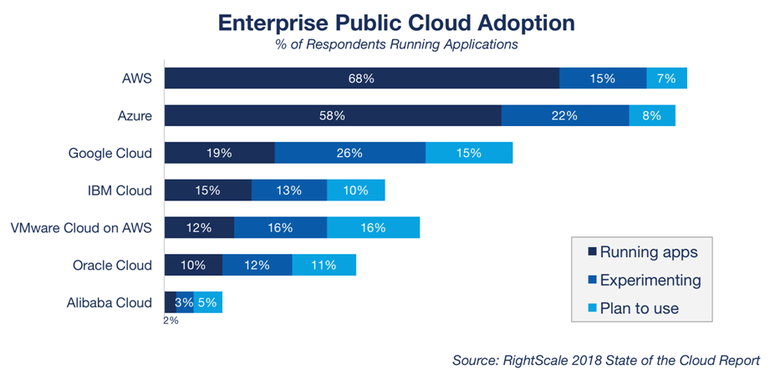
\includegraphics[width=\columnwidth]{images/rs_cloudComp.png}
\caption{Vergleich Cloud-Dienstleister auf der Basis gehosteter Applikationen}
\label{fig:cloudProvComp}
\end{figure}

Aufgrund der gezeigten Ergebnisse und der Benchmarks von \textit{DNSPref} wurden nun die Cloud-Anbieter festgelegt. Die zur Erstellung des Modells untersuchten DNS-Services lauten wie folgt:

\begin{tabular}{lll}
\raisebox{-.5\height}{
\includegraphics[width=55pt]{images/logo_aws.png}} & Amazon Web Services - Route 53 \\
\raisebox{-.5\height}{
\includegraphics[width=60pt]{images/logo_azure2.png}} & Microsoft Azure - DNS-Zonen \\ \\
\raisebox{-.5\height}{
\includegraphics[width=55pt]{images/logo_google.png}} & Google Cloud DNS\\ 
\\
\end{tabular}
\section{Das Modell}
Im folgenden Abschnitt soll das in \ref{fig:ccmodel} gezeigte Modell zur Beschreibung von DNS-Cloud-Services detailliert erläutert werden. Dies soll zum Verständnis und als Hilfe bei der Anwendung dienen. Außerdem soll es die gewählte Darstellungsform und Notation beleuchten, die zur Erstellung des Modells genutzt wurde.

\begin{sidewaysfigure*}[ht]
    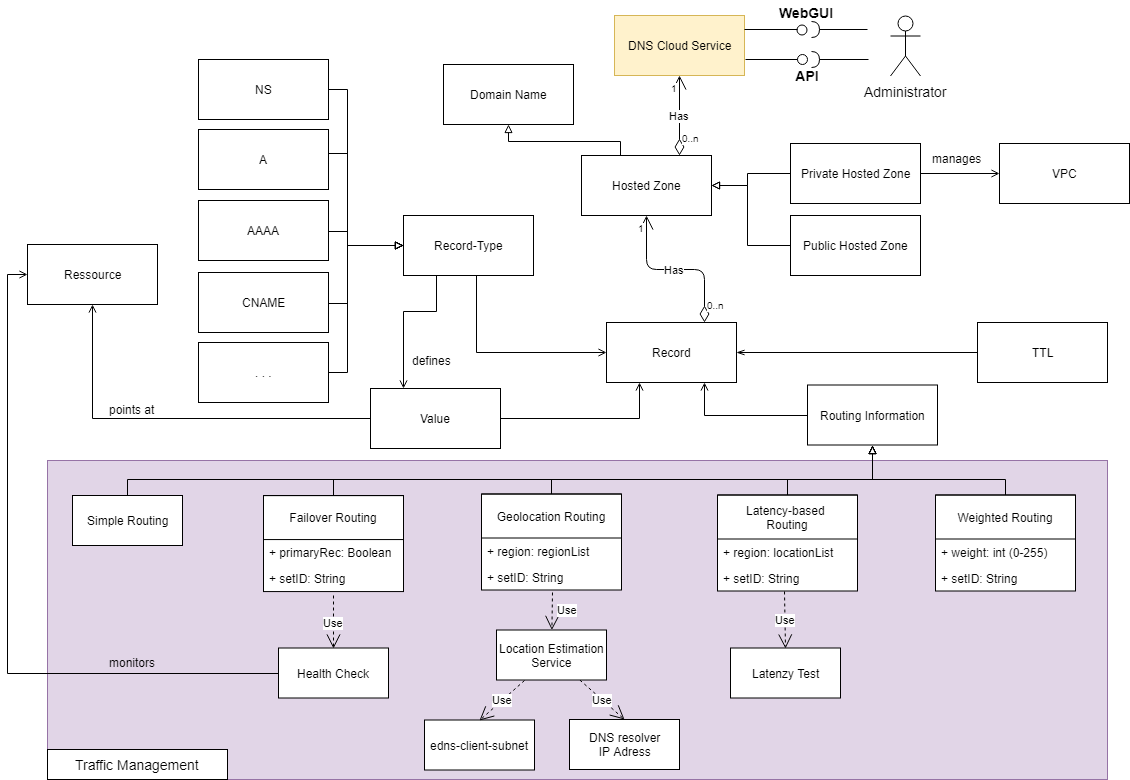
\includegraphics[width=\textwidth]{images/cc_modelxml.png}
    \caption{Modell zur Beschreibung von DNS-Cloud-Services}
    \label{fig:ccmodel}
\end{sidewaysfigure*}

\subsection{Schnittstellen}
Zur Nutzung der DNS-Cloud-Services allgemein stehen unterschiedliche Möglichkeiten zur Verfügung. Wird ein neues Benutzerkonto angelegt, geschieht dies über eine Weboberfläche. Nach der Einrichtung ist es möglich über die Benutzeroberfläche der Internetseite auf das Produktportfolio des Dienstleisters zuzugreifen. Sämtliche Interaktionen mit dem Cloud-Service sind über diese Weboberfläche möglich. So kann der Kunde jederzeit und von jedem internetfähigen Gerät, plattformunabhängig über den Browser seines Betriebssystems auf die Services zugreifen. Das bedeutet, dass keine Installation von zusätzlichen Anwendungen oder Treibern notwendig ist.

Eine weitere Möglichkeit ist der Zugriff über eine Schnittstelle zur Anwendungsprogrammierung (API). Diese Schnittstellen ermöglichen es mit der Hilfe von Kommandozeilenwerkzeugen auf die Services des Cloud-Providers zuzugreifen. Somit können auch ohne die Hilfe des Webinterfaces administrative Aufgaben bezüglich der Cloud erledigt werden. Eine API ermöglicht es ebenfalls über Skriptsprachen Routineaufgaben zu automatisieren oder den Cloud-Service in eine unternehmensinterne Software einzubinden. Dies bringt den Vorteil eines flexibleren Umgangs und einer bessere Einbindung des Cloud-Services in die alltäglichen Prozesse.

 \subsection{Hosted Zones}
Bei der Analyse der einzelnen DNS-Cloud-Dienstleistungen fällt auf, dass das zentrale Element die sogenannten Hosted-Zones darstellen. Sie dienen als Container zum Hosten der DNS-Einträge zu einer bestimmten Domäne und umschließen somit alle Informationen über die Weiterleitung des Datenverkehrs dieser.
Ein DNS-Cloud-Service kann über mehrere Hosted-Zones verfügen. Die Namensgebung findet hierbei meist über den Domain-Namen statt. Somit wird die Funktion der Hosted-Zones schnell ersichtlich. Außerdem ist über den Domain-Namen eine einzigartige Identifizierung der unterschiedlichen Zonen gewährleistet. Je nach DNS-Cloud-Dienstleistung kann jedoch auch ein abweichender Name zur betreffenden Domain gewählt werden. Laut den offiziellen Dokumenationen der Cloud-Provider, liegt das Limit an Hosted-Zones standardmäßig bei über 100 Hosted-Zones, bei allen drei untersuchten Anbietern.

\section{Fazit}
Das Domain-Name-System ist einer der wichtigsten Bestandteile der heutigen Kommunikation. Der Ausfall eines solchen Systems kann schwerwiegende Folgen für Unternehmen haben. Die Verwendung eines Cloud-Dienstes ist hier sehr sinnvoll, da diese meist über eine große globale Infrastruktur verfügen, die für eine schnelle Adressauflösung sorgen kann jedoch für einzelne Unternehmen sehr kostenintensiv im Unterhalt wäre.

Der Aufbau der verschiedenen untersuchten Cloud-Dienste weicht nicht weit voneinander ab und auch die Leistungsunterschiede und preisliche Differenz ist nicht übermäßig relevant. Das erstellte Modell bildet die Kernfunktionalitäten der unterschiedlichen DNS-Cloud-Dienste ab. Es ermöglicht Nutzern eine bessere Übersicht über die Funktionen und den Aufbau eines solchen Services. 

\subsection{Persönliche Errungenschaften}
Während der Erstellung des Modells hatte ich die Möglichkeit mich näher mit dem Thema DNS und Cloud-Dienste zu beschäftigen. Aufgrund meines geringen Vorwissens konnte ich viel über die beiden Themenbereiche lernen und auch erste praktische Erfahrungen im Umgang mit Cloud-Services sammeln. Da ich im Voraus ebenfalls wenig Expertise in der Erstellung von Modellen hatte, konnte ich diese an einem praktischen und angewandten Beispiel ebenfalls vertiefen.


\bibliographystyle{IEEEtran}
\bibliography{xliteratur}




% trigger a \newpage just before the given reference
% number - used to balance the columns on the last page
% adjust value as needed - may need to be readjusted if
% the document is modified later
%\IEEEtriggeratref{8}
% The "triggered" command can be changed if desired:
%\IEEEtriggercmd{\enlargethispage{-5in}}

% references section

% can use a bibliography generated by BibTeX as a .bbl file
% BibTeX documentation can be easily obtained at:
% http://mirror.ctan.org/biblio/bibtex/contrib/doc/
% The IEEEtran BibTeX style support page is at:
% http://www.michaelshell.org/tex/ieeetran/bibtex/
%\bibliographystyle{IEEEtran}
% argument is your BibTeX string definitions and bibliography database(s)
%\bibliography{IEEEabrv,../bib/paper}
%
% <OR> manually copy in the resultant .bbl file
% set second argument of \begin to the number of references
% (used to reserve space for the reference number labels box)



%\begin{thebibliography}{1}

%\bibitem{IEEEhowto:kopka}
%H.~Kopka and P.~W. Daly, \emph{A Guide to \LaTeX}, 3rd~ed.\hskip 1em plus
%  0.5em minus 0.4em\relax Harlow, England: Addison-Wesley, 1999.
%
%\end{thebibliography}


\end{document}


